%------------------------------------------------------------------------------
%	CAPITOLO 15
%------------------------------------------------------------------------------

\chapter{Alt, chi va là}
\index[Personaggi]{Bigano (fabbro)}Bigano, fabbro di professione, era un acceso liberale del 1859, mangiacristi e mangiapreti, fremeva per poter trasportare l'incudine sull'altar maggiore, diceva. Caporale della guardia nazionale si scalmanava da vero bravaccio\footnote{Chi con parole e portamento minacciosi e arroganti cerca di imporsi più all'attenzione che alla volontà altrui}.\\
\indent Una sera del Maggio 1859 era caporale caposto al quartiere della guardia nazionale, nel Corso e nella casa ex caserma dei gendarmi pontefici, poi Lugaresi, De Maria, ora \index[Luoghi]{Lugaresi (palazzo)}Dopolavoro\footnote{\textbf{Palazzo Lugaresi} era in corso Garibaldi, non lontano dal Credito Romagnolo. Era l'antico palazzo del Cav. Aristide Lugaresi, farmacista e consigliere comunale, padre di Santina e nonno materno di Antonio Camanzi, che ne divenne l'unico erede negli anni '30. Rimase distrutto durante la seconda guerra mondiale}.\\Ad un tratto sentì uno scalpittio di cavallo che veniva dal \index[Luoghi]{Ponte Nuovo}pontenuovo\footnote{Si tratta del ponte sulla via Reale, all'incrocio con corso Garibaldi}. Il caldanzoso caporale, fu pronto, al buio, a gridare:\\
\indent "Alt chi va là".\\
\indent Rispose una voce: "Ufficiale austriaco".\\
\indent Non ci volle altro, senza di nulla più curarsi il nostro valoroso caporale, abbandonò armi, berretto e via di corsa per la porta di dietro per i campi, subito imitato dai suoi militi. Si fece vedere solamente quando la burrasca fu passata da qualche giorno.\\
\indent Chi era stato? All'insaputa di tutti e senza preavvisi era arrivata l'avanguardia austriaca, della intera guarnigione di Ancona, che aveva sgombrato della fortezza per recarsi sui campi Lombardi alla guerra.\\
\indent Per chi non lo sapesse il corpo austriaco era forte di seimila uomini, aveva disposto l'avanguardia alla \index[Luoghi]{Tosca}Tosca\footnote{Zona a ridosso dell'incrocio tra Via Reale e Via Valeria}, sul \index[Luoghi]{Ponte Nuovo}Ponte Nuovo vari pezzi di cannone ai quali erano addetti gli artiglieri sempre con la miccia accesa e pronti al fuoco.\\
\indent Figurarsi il terrore della popolazione allo spettacolo insolito, molto di più perché gli austriaci si erano fissati che in Alfonsine fosse nascosto \index[Personaggi]{Garibaldi Giuseppe}Garibaldi e lo cercavano affannosamente. \\
\indent Si dice anche che un tale, sfuggito alla memoria, alle minacce di un austriaco, fece finta di soddisfarlo, lo condusse nella sosta del fiume, se lo fece camminare innanzio e quando fu ai limiti della scarpata, con una spinta lo mandò a ruzzolare nell'acqua e fuggì a gambe levate per sottrarsi al pericolo.\\
\indent Il generale austriaco dormì nella \index[Luoghi]{Lugaresi (palazzo)}casa Lugaresi.\\
\indent Furono requisiti generi, carri, carrettieri e contadini per trasportare gli equipaggiamenti e servizi austriaci fino all'altra tappa di \index[Luoghi]{Argenta}Argenta.

 \begin{figure}[htb]
    \centering
    %\vspace{-0.7cm}
    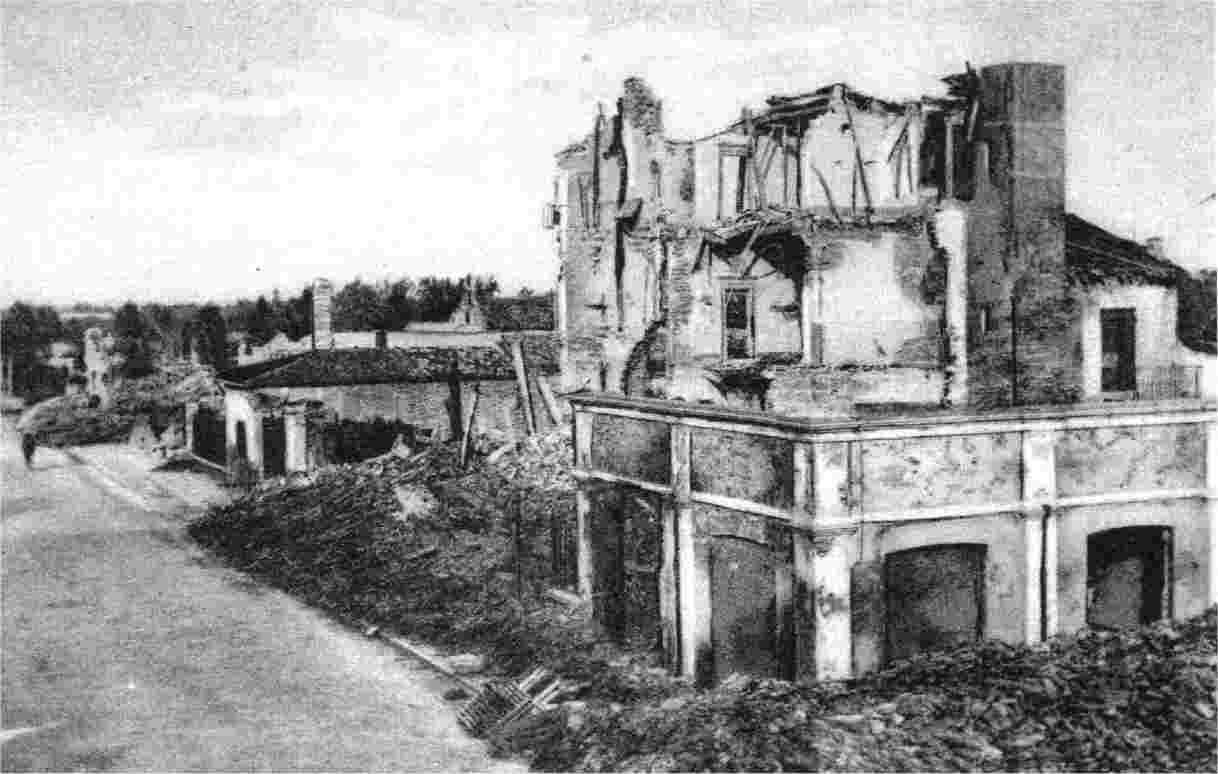
\includegraphics[width=\textwidth]{palazzolugaresi}
    \caption{Palazzo Lugaresi distrutto dopo la guerra.\label{fig:palazzolugaresi}}
    %\vspace{-0.3cm}
\end{figure}
